\chapter{Results}
\label{chap:partI_results}

After the training, the four competing architectures and the non-ML baseline are compared in three different scenarios: full design, weight maps only (no AO) and artifacts oversampling only (no WM). 
The 70 full-size images of the test set are used as a testbed.
\Cref{tab:metrics} reports individual model performances in terms of both detection and counting ability.
\begin{table}[H]
\centering
\resizebox{\textwidth}{!}{\begin{tabular}{lr|rrrrr|rrrr}
\toprule
Model &  Threshold &      $\boldsymbol{F_1 }$ & \textbf{AUC} & Accuracy &  Precision &  Recall & $\boldsymbol{R^2}$ &  \textbf{MAE} &  MedAE &     MPE (\%) \\
\midrule
\textbf{c-ResUnet}          &      \textbf{0.875} &  \underline{\textbf{0.8149}} & \underline{\textbf{0.8705}} &    \textbf{0.6877} &     0.9081 &  \textbf{0.7391} & \underline{\textbf{0.8215}} &  \underline{\textbf{3.0857}} &    \textbf{1.0} & -5.13 \\
c-ResUnet (no AO)  &      0.875 &  0.8047 & 0.8741 &    0.6732 &     0.9019 &  0.7264 & 0.8077 &  3.0857 &    1.5 & -6.24 \\
c-ResUnet (no WM)  &      0.875 &  0.7613 & 0.8594 &    0.6147 &     0.9418 &  0.6389 & 0.7048 &  3.6857 &    \textbf{1.0} & -19.14 \\
\midrule
ResUnet            &      0.850 &  0.7855 & 0.8579 &    0.6468 &     0.8865 &  0.7052 & 0.7831 &  3.3286 &    \textbf{1.0} & \textbf{-4.84}  \\
ResUnet (no WM)    &      0.850 &  0.7513 & 0.8643 &    0.6016 &     0.9387 &  0.6262 & 0.6955 &  4.0571 &    2.0 & -24.12 \\
Unet               &      0.875 &  0.7724 & 0.8609 &    0.6291 &     0.9117 &  0.6700 & 0.7560 &  3.5143 &    1.5 & -14.36 \\
Unet (no WM)       &      0.850 &  0.7886 & 0.8461 &    0.6510 &     0.8989 &  0.7024 & 0.8069 &  3.1571 &    2.0 & -9.23 \\
small Unet         &      0.875 &  0.7563 & 0.8691 &    0.6081 &     0.9264 &  0.6389 & 0.7682 &  3.5714 &    2.0 & -21.37 \\
small Unet (no WM) &      0.825 &  0.6697 & 0.8326 &    0.5034 &     \textbf{0.9483} &  0.5176 & 0.5723 &  4.7714 &    2.0 & -32.01 \\
\midrule
Adaptive Threshold &      0.994 & 0.6106 & 0.0865 &	0.4394 &	0.5680 &	0.6601  & 0.3565 &	8.0143 &	6.0 &	78.26 \\
\bottomrule
\end{tabular}}
\caption{\textbf{Performance metrics.}
Test set performance using the optimal \textit{kneed} threshold. The first five columns report the detection metrics, while the latter ones evaluate counting performance.
}
\label{tab:metrics}
% \end{center}
\end{table}

% \noindent\textbf{Performance}.
\section{Performance}

% By looking at the main figures of merit ($F_1$ score and MAE), it is clear how deep learning approaches perform better than the adaptive thresholding.
As a first observation, it is soon apparent how deep learning approaches perform better than adaptive thresholding according to all the considered metrics.

Starting with detection performance,
% as measured principally through the $F_1$ and AUC scores,
c-ResUnet clearly outperforms all competitors in terms of $F_1$ score.
% c-ResUnet clearly outperforms all competitors.
Remarkably, the Unet is consistently worse than c-ResUnet and ResUnet despite having far more parameters (nearly 14M against 1.7M and 887k, respectively).
The advantage of the ResUnet architectures is even more evident with respect to the lighter Unet version which has a comparable number of parameters (876k).
The values of the area under the precision/recall curves also confirm this supremacy. While the $F_1$ can be interpreted as a measure of maximum performance achieved, the AUC can be even more powerful since it indicates a global measure of performance independent of the choice of the threshold for binarization (see \cref{fig:results:PR}). Again, c-ResUnet sits on top of the list, with ResUnet and Unet following shortly after. Interestingly, the small Unet performs on par according to the AUC metrics, suggesting that the choice of the threshold is perhaps suboptimal for the test set.
\begin{figure}
    \centering
    \includegraphics[width=\textwidth]{figures/140_results/PR_test.pdf}
    \caption{\textbf{Precision/Recall plot.} 
    Test set precision/recall curves varying the threshold for predicted heatmap binarization. The inset plot reports a zoom of the top right corner to highlight differences of the various curves.}
    \label{fig:results:PR}
\end{figure}

In addition, c-ResUnet keeps its leading role also when extending the evaluation to the other metrics.
The only meaningful exception is precision, for which the Unet architectures are better. This is probably due to a tendency to overdetection. 
Nonetheless, the ResUnet counterparts well balance this behaviour with a significant improvement in accuracy and recall.

c-ResUnet remains the most accurate model also when shifting the focus on counting performance. Although the difference is hardly noticeable concerning the MAE, the gap becomes more prominent when looking at the $R^2$, with the \mbox{c-ResUnet} reaching a decent value of roughly 82\% of explained variability.
Interestingly, this time the ranking between ResUnet and Unet is inverted, with the latter performing slightly better in terms of counting.

Finally, it is worth noticing that adopting the kneed optimal threshold ensures large cutoffs and enforces only detections with high confidence.
Although desired, this behavior also increases false negatives as less cells are detected. 
As a result, we observe a drop in the accuracy whereby the impact of false negatives is twice as much the one in the $F_1$ score (cf. \cref{eq:accuracy,eq:F1}), thus explaining the gap between these two metrics.
% As a result, we observe a drop in the measures that are more impacted by false negatives, which explains the lower value of the accuracy compared to the $F_1$ score.
In conclusion, the model provides reliable predictions and satisfies the design requirement of being conservative with counts, as suggested by the negative values of MPE for all experimental conditions.

\begin{figure}[!b]
% \begin{wrapfigure}{R}{0.55\textwidth}
\centering
\includegraphics[width=\textwidth]{figures/130_methods/weigths_effect.png}
\caption{\textbf{Weight map effect.} 
Predicted heatmaps obtained with c-ResUnet (top row) and c-ResUnet (no WM).} 
\label{fig:weigths_effect}
% \end{wrapfigure}
\end{figure}
\section{Design evaluation}

This section presents the comparison of the different design choices investigated through the ablation studies.
In order to evaluate the impact of artifacts oversampling and weight maps, the experiments were repeated under the same conditions described in \cref{sec:model_training}, alternately switching off one of the two design choices.

From \cref{tab:metrics} it is evident how penalizing errors in crowded areas generally has a positive impact. Indeed, experiments exploiting weight maps achieve consistently better results than those without this addition (no WM). The only exceptions are the Unet and ResUnet architectures -- the former in terms of $F_1$ score, MAE and $R^2$, and the latter concerning AUC.  
In particular, this strategy seems to produce a loss in precision to foster a more significant gain in accuracy and recall.
\Cref{fig:weigths_effect} illustrates a visual comparison of the c-ResUnet output in crowded areas with (top) and without (bottom) weight maps. 
Again, its beneficial contribution is apparent, with close-by cells sharply separated when exploiting the weight maps.

Regarding the impact of artifacts augmentation, \cref{tab:metrics} shows how there is little difference between the full c-ResUnet and the one without oversampling of challenging examples (no AO).
In particular, the advantage of artifacts oversampling is numerically minimal.
This is also confirmed by qualitative evaluation (\cref{fig:predictions}).
On the one hand, the c-ResUnet (no AO) avoids detecting more evident biological artifacts as the stripe  in \cref{fig:predictions:noAO} even without specific oversampling.
On the other, the c-ResUnet  still fails to ignore the macaroni-shaped accumulation of fluorophore (\cref{fig:predictions:artifact}) although additional challenging examples are provided during training.
Probably, this is due to the lack of similar structures in the training set, which makes the oversampling ineffective for such kind of artifacts.
For this reason, the experiment was not replicated for the other architectures. 
% \begin{figure}
% \centerline{
%      \begin{subfigure}[]{0.55\textwidth}
%          \centering
% \includegraphics[width=\textwidth]{figures/140_results/pred_ResUnet_noAO:281.pdf}
%         \caption{
%         % c-ResUnet (no AO) prediction on artifact
%         }
%         \label{fig:predictions:noAO}
%      \end{subfigure}
%           \begin{subfigure}[]{0.55\textwidth}
%          \centering
% \includegraphics[width=\textwidth]{figures/140_results/pred_ResUnet:254.pdf}
%         \caption{
%         % c-ResUnet prediction on artifact
%         }
%         \label{fig:predictions:artifact}
%      \end{subfigure}
% }
% \centerline{
%           \begin{subfigure}[]{0.55\textwidth}
%          \centering
% 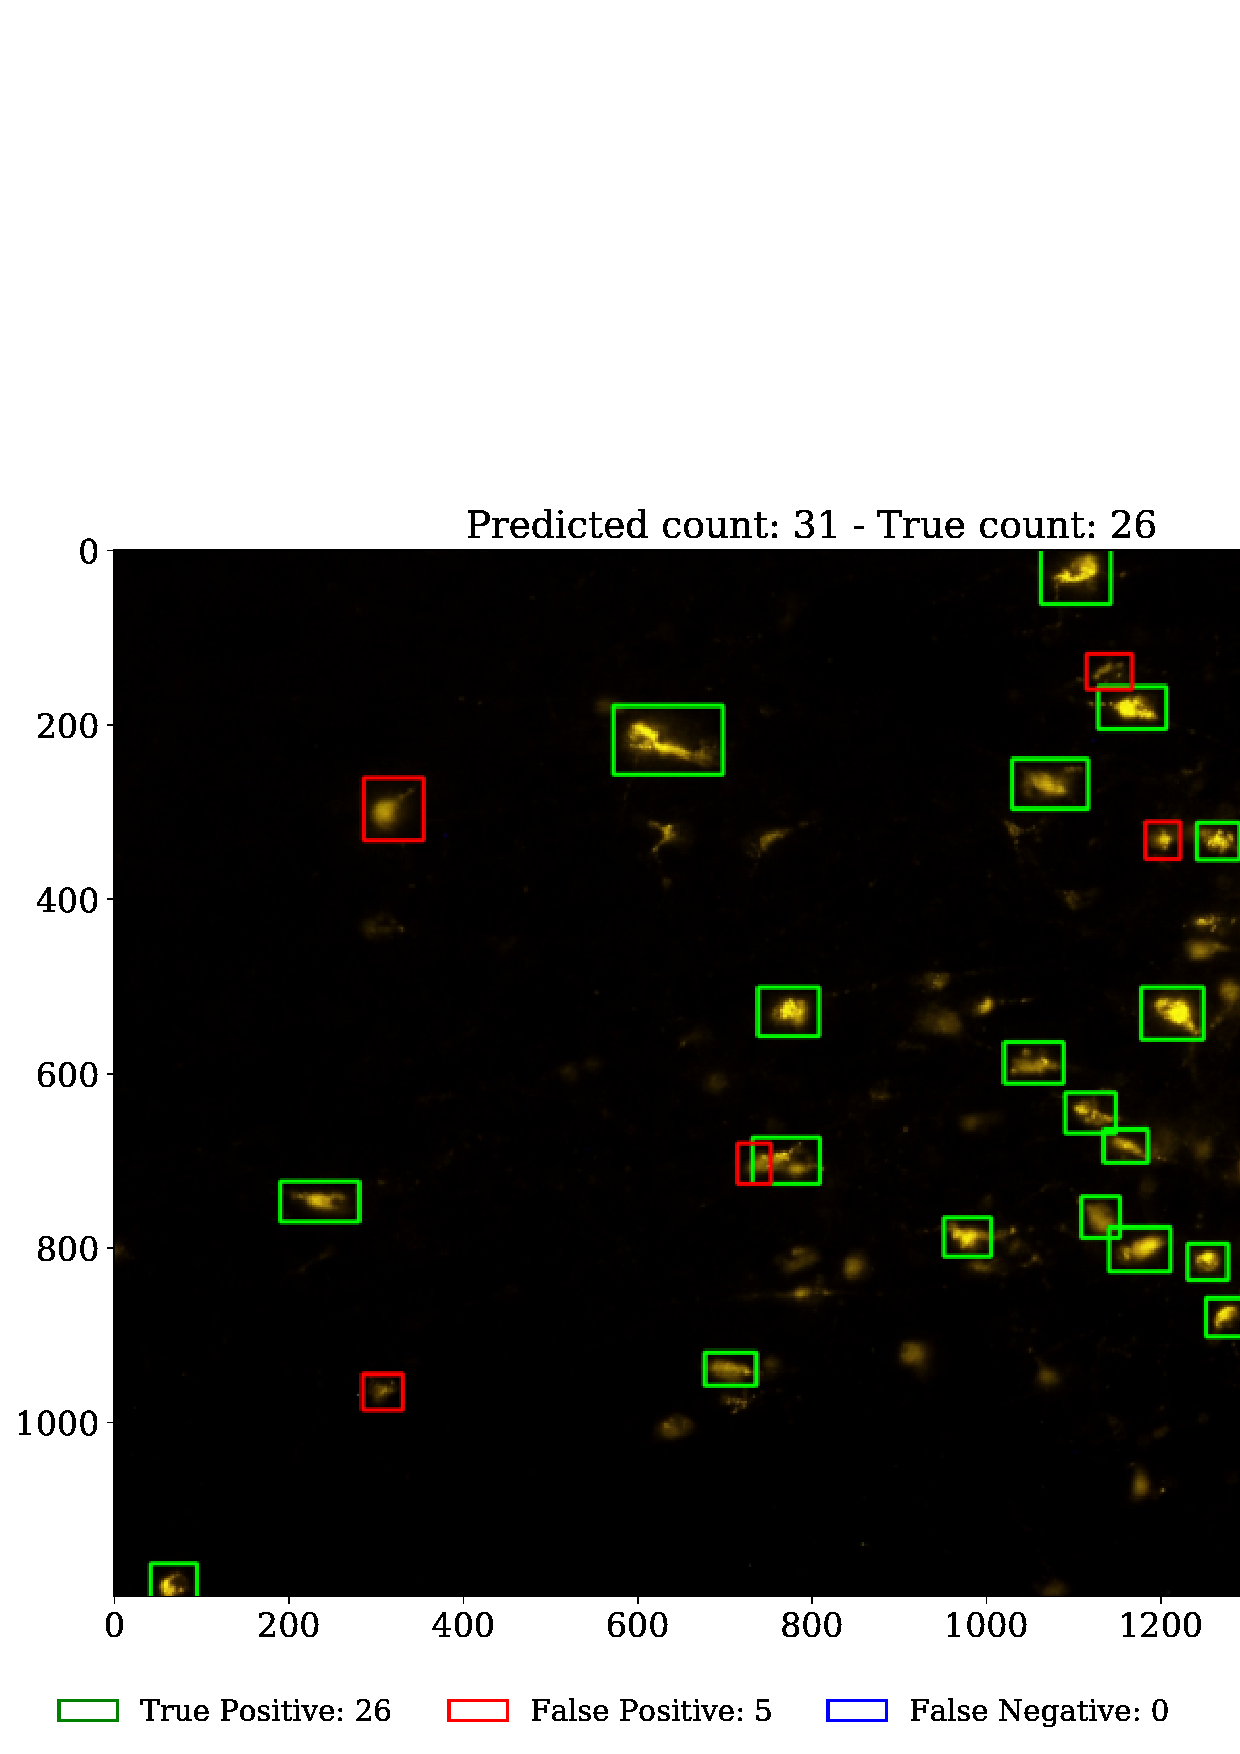
\includegraphics[width=\textwidth]{figures/140_results/pred_ResUnet:168.pdf}
%         \caption{
%         % c-ResUnet prediction on artifact
%         }
%         \label{fig:predictions:false-positives}
%      \end{subfigure}
%       \begin{subfigure}[]{0.55\textwidth}
%          \centering
% \includegraphics[width=\textwidth]{figures/140_results/pred_ResUnet:278.pdf}
%         \caption{
%         % c-ResUnet prediction on artifact
%         }
%         \label{fig:predictions:false-negatives}
%      \end{subfigure}
% }
% \caption{\textbf{Results on test images}. 
% % Top row illustrates AO effect. 
% The c-ResUnet (no AO) correctly handles the evident stripe in the top left corner (\hyperref[fig:predictions:noAO]{a}), while the c-ResUnet fails with the macaron-shaped artifact (\hyperref[fig:predictions:artifact]{b}).
% % Bottom row highlights c-ResUnet predictive ability. 
% Also, notice how false positives (\hyperref[fig:predictions:false-positives]{c}, red boxes) look like target cells. Likewise, the objects discarded (\hyperref[fig:predictions:false-negatives]{d}, blue boxes) are similar to other stains that were not annotated.
% } 
% \label{fig:predictions}
% \end{figure}

% \savegeometry{origigeom}
% \clearpage
% \newgeometry{lmargin=1.5cm}
% \begin{landscape}
% \begin{figure}[!b]
%     \centering
%     \subfloat[\textit{Challenges:}
%     ]{
%     \includegraphics[width=\linewidth]{figures/140_results/pred_ResUnet:254.pdf}\label{fig:artifacts:clumping}
%     }
%     \caption{\textbf{Challenges and artifacts.}}
%     \label{fig:artifacts}
% \end{figure}%

% \begin{figure}[ht]\ContinuedFloat
%     \centering
%     \subfloat[\textit{Biological artifacts:} 
%     ]{
%     \includegraphics[width=\linewidth]{figures/120_dataset/challenges/stripe_and_filaments.pdf}\label{fig:artifacts:stripe}
%     }
%     \caption{\textbf{Challenges and artifacts. (2)}}
% \end{figure}%
% % \end{landscape}

% % \begin{landscape}
% \begin{figure}[ht]\ContinuedFloat
%     \centering
%     \subfloat[\textit{Technical artifacts:}
%     ]{\includegraphics[width=\linewidth]{figures/120_dataset/challenges/artifacts.pdf}\label{fig:artifacts:macaroon}
%     }
%     \caption{\textbf{Challenges and artifacts. (3)}}
% \end{figure}
% \end{landscape}
% \clearpage
% \restoregeometry


% \savegeometry{origigeom}
% \clearpage
% \newgeometry{lmargin=1.5cm}
% \begin{landscape}

% \begin{figure}[!b]
% \centering
% \subfloat[]{
% \includegraphics[width=\linewidth]{figures/140_results/pred_ResUnet_noAO:281.pdf}\label{fig:predictions:noAO}
% }
% \caption{\textbf{Results on test images}. 
% % Top row illustrates AO effect. 
% The c-ResUnet (no AO) correctly handles evident artifacts (\ref{fig:predictions:noAO}, top left corner), while the c-ResUnet fails with more problematic structures (\ref{fig:predictions:artifact}).
% % Bottom row highlights c-ResUnet predictive ability. 
% Notice how false positives (\ref{fig:predictions:false-positives}, red boxes) look like target cells. Likewise, the objects discarded (\ref{fig:predictions:false-negatives}, blue boxes) are similar to other stains that were not annotated.
% } 
% \label{fig:predictions}
% \end{figure}
% \begin{figure}[ht]\ContinuedFloat
% \centering

% \subfloat[]{
% \includegraphics[width=\linewidth]{figures/140_results/pred_ResUnet:254.pdf}\label{fig:predictions:noAO}
% }
% \caption{\textbf{Results on test images}. 
% % Top row illustrates AO effect. 
% The c-ResUnet (no AO) correctly handles evident artifacts (\ref{fig:predictions:noAO}, top left corner), while the c-ResUnet fails with more problematic structures (\ref{fig:predictions:artifact}).
% % Bottom row highlights c-ResUnet predictive ability. 
% Notice how false positives (\ref{fig:predictions:false-positives}, red boxes) look like target cells. Likewise, the objects discarded (\ref{fig:predictions:false-negatives}, blue boxes) are similar to other stains that were not annotated.
% } 
% \label{fig:predictions}
% \end{figure}


% \begin{figure}[ht]\ContinuedFloat
% \centering
% \subfloat[]{
% 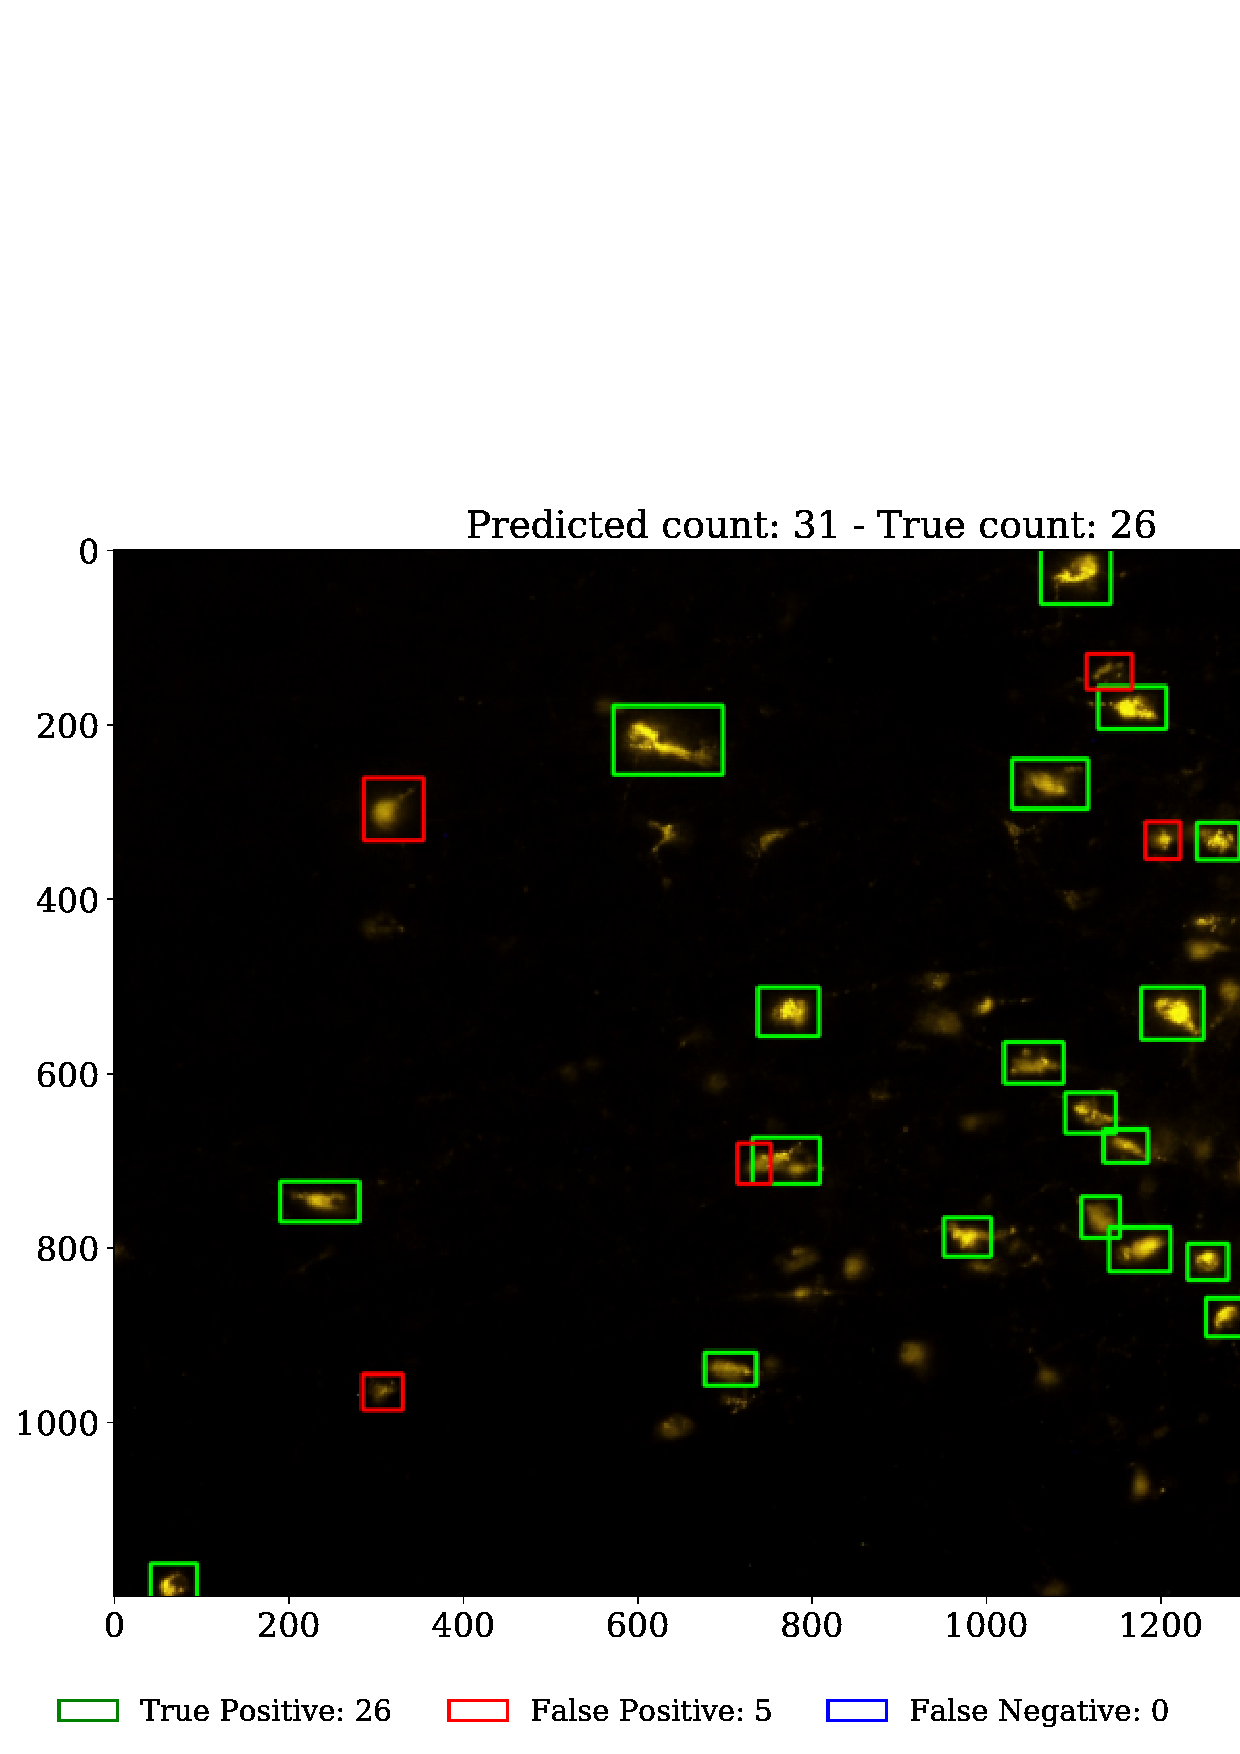
\includegraphics[width=\linewidth]{figures/140_results/pred_ResUnet:168.pdf}\label{fig:predictions:noAO}
% }
% \caption{\textbf{Results on test images}. 
% % Top row illustrates AO effect. 
% The c-ResUnet (no AO) correctly handles evident artifacts (\ref{fig:predictions:noAO}, top left corner), while the c-ResUnet fails with more problematic structures (\ref{fig:predictions:artifact}).
% % Bottom row highlights c-ResUnet predictive ability. 
% Notice how false positives (\ref{fig:predictions:false-positives}, red boxes) look like target cells. Likewise, the objects discarded (\ref{fig:predictions:false-negatives}, blue boxes) are similar to other stains that were not annotated.
% } 
% \label{fig:predictions}
% \end{figure}


% \begin{figure}[ht]\ContinuedFloat
% \centering
% \subfloat[]{
% \includegraphics[width=\linewidth]{figures/140_results/pred_ResUnet:278.pdf}\label{fig:predictions:noAO}
% }
% \caption{\textbf{Results on test images}. 
% % Top row illustrates AO effect. 
% The c-ResUnet (no AO) correctly handles evident artifacts (\ref{fig:predictions:noAO}, top left corner), while the c-ResUnet fails with more problematic structures (\ref{fig:predictions:artifact}).
% % Bottom row highlights c-ResUnet predictive ability. 
% Notice how false positives (\ref{fig:predictions:false-positives}, red boxes) look like target cells. Likewise, the objects discarded (\ref{fig:predictions:false-negatives}, blue boxes) are similar to other stains that were not annotated.
% } 
% \label{fig:predictions}
% \end{figure}

% \end{landscape}

% \clearpage
% \restoregeometry




\begin{figure}[!b]
\centering
\subfloat[stripes and filaments]{
\includegraphics[width=\textwidth]{figures/140_results/pred_ResUnet_noAO:281.pdf}\label{fig:predictions:noAO}
}
\caption{\textbf{Results on test images}. 
The c-ResUnet (no AO) correctly handles the evident stripe in the top left corner despite not receiving dedicated oversampling for such biological structures
% Filaments are also correctly interpreted
} 
\label{fig:predictions}
\end{figure}
\begin{figure}[ht]\ContinuedFloat
\centering

\subfloat[technical artifacts]{
\includegraphics[width=\textwidth]{figures/140_results/pred_ResUnet:254.pdf}\label{fig:predictions:artifact}
}
\caption{\textbf{Results on test images (2)}. 
The c-ResUnet fails with the \mbox{macaron-shaped} artifact in the middle of the picture, suggesting that the oversampling strategy is not effective in this case. However, notice that no other similar artifacts are present in the training set
} 
\end{figure}


\begin{figure}[ht]\ContinuedFloat
\centering
\subfloat[false positives]{
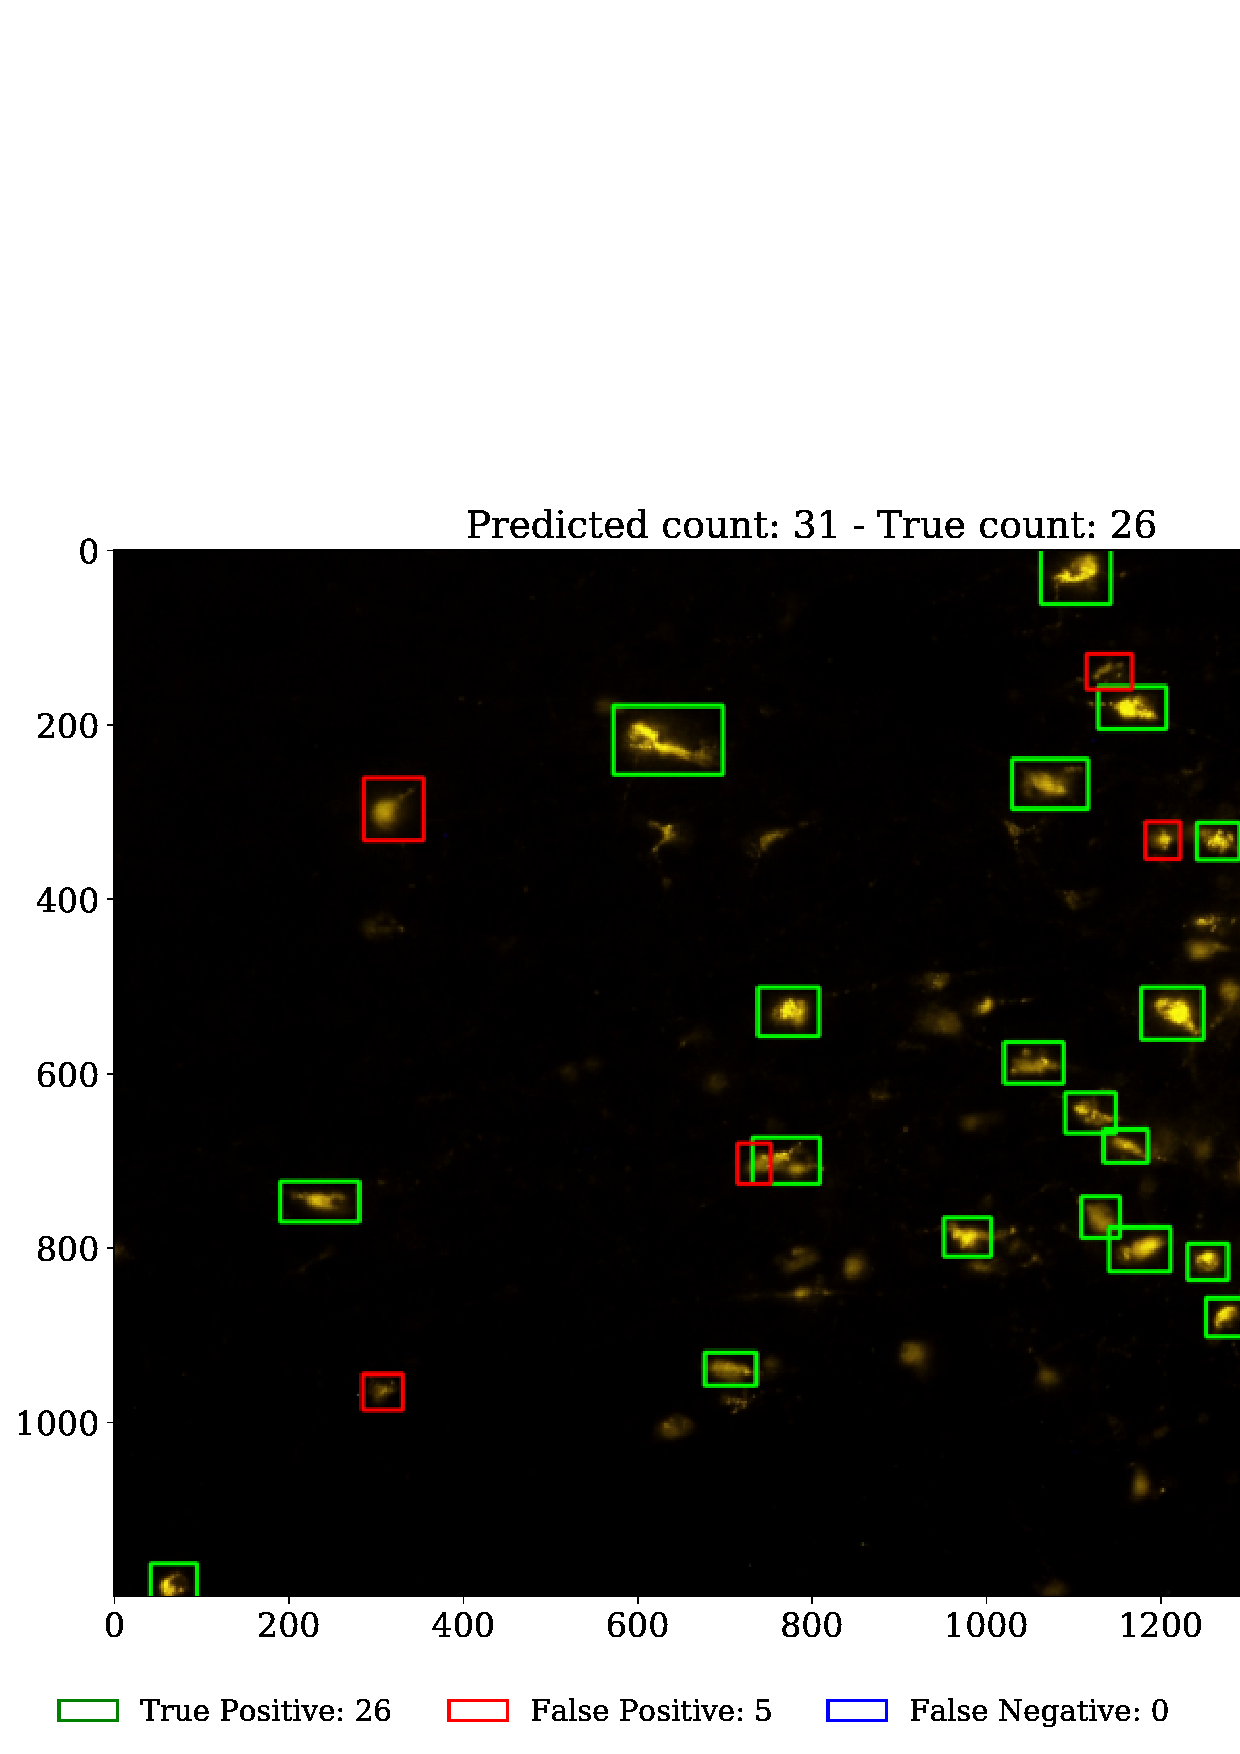
\includegraphics[width=\textwidth]{figures/140_results/pred_ResUnet:168.pdf}\label{fig:predictions:false-positives}
}
\caption{\textbf{Results on test images (3)}. 
The c-ResUnet sometimes produces false positives (red boxes), i.e. it labels as cell structures that are not annotated by the researcher.
However, the difference with marked cells is marginal (cf. also with \hyperref[fig:predictions:false-negatives]{d}), suggesting that these errors may lie within the limits of arbitrariness intrinsic to the task
} 
\end{figure}


\begin{figure}[ht]\ContinuedFloat
\centering
\subfloat[false negatives]{
\includegraphics[width=\textwidth]{figures/140_results/pred_ResUnet:278.pdf}\label{fig:predictions:false-negatives}
}
\caption{\textbf{Results on test images (4)}. 
% Top row illustrates AO effect. 
The c-ResUnet is generally conservative in predictions, thus generating false positives (blue boxes).
However, these are similar to other stains that were not annotated (cf. also with \hyperref[fig:predictions:false-positives]{c}), thus falling again within the limits of operator's interpretation
} 
\end{figure}









% \savegeometry{origigeom}
% \clearpage
% \newgeometry{lmargin=1.5cm}


% \begin{figure}[!b]
% \centering
% \subfloat[]{
% \includegraphics[width=\textwidth]{figures/140_results/pred_ResUnet_noAO:281.pdf}\label{fig:predictions:noAO}
% }
% \caption{\textbf{Results on test images}. 
% % Top row illustrates AO effect. 
% The c-ResUnet (no AO) correctly handles evident artifacts (\ref{fig:predictions:noAO}, top left corner), while the c-ResUnet fails with more problematic structures (\ref{fig:predictions:artifact}).
% % Bottom row highlights c-ResUnet predictive ability. 
% Notice how false positives (\ref{fig:predictions:false-positives}, red boxes) look like target cells. Likewise, the objects discarded (\ref{fig:predictions:false-negatives}, blue boxes) are similar to other stains that were not annotated.
% } 
% \label{fig:predictions}
% \end{figure}
% \begin{figure}[ht]\ContinuedFloat
% \centering

% \subfloat[]{
% \includegraphics[width=\textwidth]{figures/140_results/pred_ResUnet:254.pdf}\label{fig:predictions:noAO}
% }
% \caption{\textbf{Results on test images}. 
% % Top row illustrates AO effect. 
% The c-ResUnet (no AO) correctly handles evident artifacts (\ref{fig:predictions:noAO}, top left corner), while the c-ResUnet fails with more problematic structures (\ref{fig:predictions:artifact}).
% % Bottom row highlights c-ResUnet predictive ability. 
% Notice how false positives (\ref{fig:predictions:false-positives}, red boxes) look like target cells. Likewise, the objects discarded (\ref{fig:predictions:false-negatives}, blue boxes) are similar to other stains that were not annotated.
% } 
% \label{fig:predictions}
% \end{figure}


% \begin{figure}[ht]\ContinuedFloat
% \centering
% \subfloat[]{
% 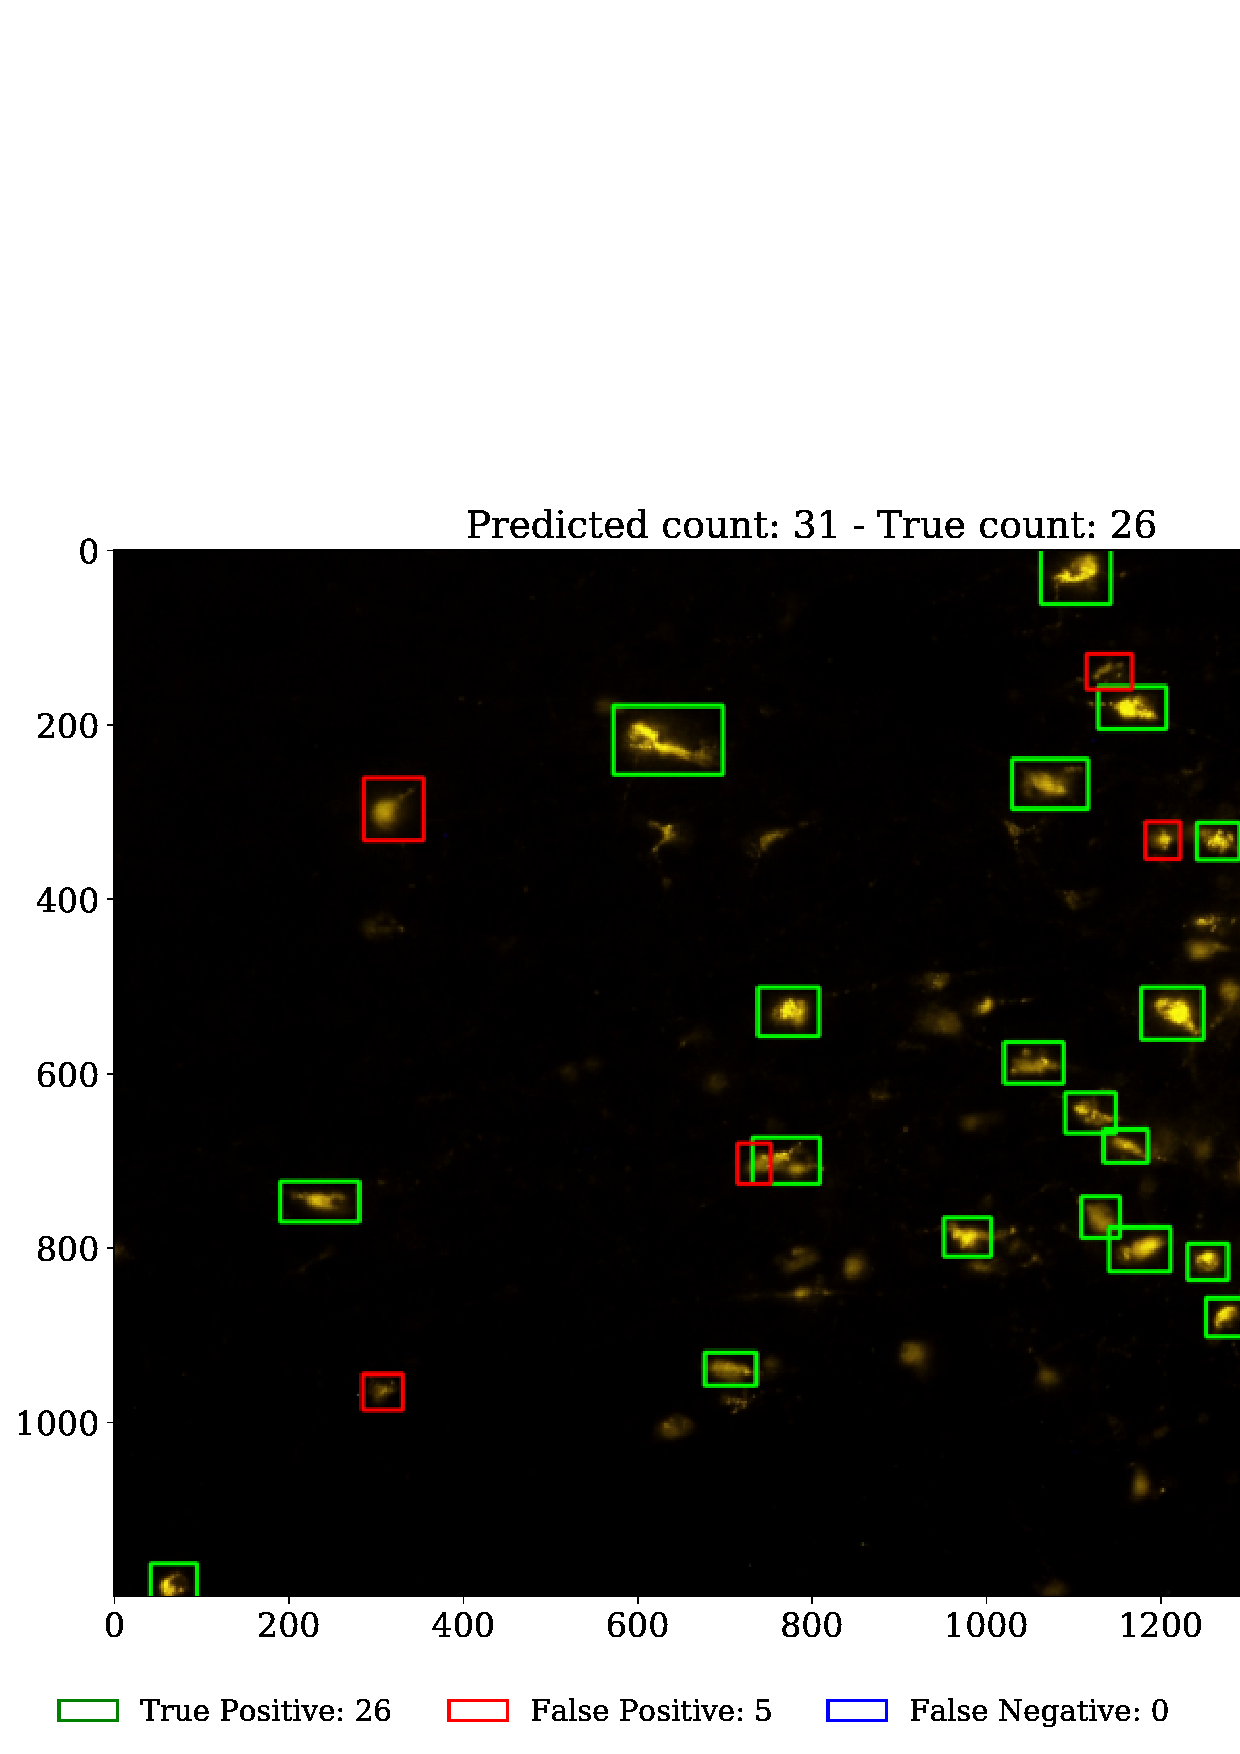
\includegraphics[width=\textwidth]{figures/140_results/pred_ResUnet:168.pdf}\label{fig:predictions:noAO}
% }
% \caption{\textbf{Results on test images}. 
% % Top row illustrates AO effect. 
% The c-ResUnet (no AO) correctly handles evident artifacts (\ref{fig:predictions:noAO}, top left corner), while the c-ResUnet fails with more problematic structures (\ref{fig:predictions:artifact}).
% % Bottom row highlights c-ResUnet predictive ability. 
% Notice how false positives (\ref{fig:predictions:false-positives}, red boxes) look like target cells. Likewise, the objects discarded (\ref{fig:predictions:false-negatives}, blue boxes) are similar to other stains that were not annotated.
% } 
% \label{fig:predictions}
% \end{figure}


% \begin{figure}[ht]\ContinuedFloat
% \centering
% \subfloat[]{
% \includegraphics[width=\textwidth]{figures/140_results/pred_ResUnet:278.pdf}\label{fig:predictions:noAO}
% }
% \caption{\textbf{Results on test images}. 
% % Top row illustrates AO effect. 
% The c-ResUnet (no AO) correctly handles evident artifacts (\ref{fig:predictions:noAO}, top left corner), while the c-ResUnet fails with more problematic structures (\ref{fig:predictions:artifact}).
% % Bottom row highlights c-ResUnet predictive ability. 
% Notice how false positives (\ref{fig:predictions:false-positives}, red boxes) look like target cells. Likewise, the objects discarded (\ref{fig:predictions:false-negatives}, blue boxes) are similar to other stains that were not annotated.
% } 
% \label{fig:predictions}
% \end{figure}

% \clearpage
% \restoregeometry